\documentclass[twocolumn,twoside]{Jornadas}
\usepackage[latin1]{inputenc}
\usepackage[dvips]{epsfig}
\usepackage[]{ulem}
\usepackage[]{algorithmic}
%\usepackage{graphicx}
\usepackage{epstopdf}
\usepackage[lofdepth,lotdepth]{subfig}

\def\BibTeX{{\rm B\kern-.05em{\sc i\kern-.025em b}\kern-.08em
    T\kern-.1667em\lower.7ex\hbox{E}\kern-.125emX}}

\newtheorem{theorem}{Teorema}
\newtheorem{mydef}{Definition}

\hyphenation{pa-ra-le-lis-mo pro-cee-dings de-ma-sia-do Su-ge-ri-mos
             mo-di-fi-ca-cio-nes afi-lia-cio-nes re-fe-ren-te co-men-ta-rios
             usan-do pro-ble-ma plan-ti-lla}

\begin{document}
\title{Parallelization of whole genome alignment}
\author{%
     Julio C\'esar Garc\'ia Vizca\'ino%
     \thanks{Dpto. de Arquitectura de Computadores y Sistemas Operativos, e-mail: {\tt juliocesar.garcia@e-campus.uab.cat.}}
     y Antonio Espinosa%
     \thanks{Dpto. de Arquitectura de Computadores y Sistemas Operativos, e-mail: {\tt antonio.espinosa@caos.uab.es.}}
}

\maketitle
\markboth{}{}
\pagestyle{empty} 
\thispagestyle{empty} % Oculta el n\'umero de la primera p\'agina

\begin{abstract} 
  With the advent of High performance computing,  it is now possible to achieve orders of magnitude performance and computation eficiency gains over conventional computer architectures. This work explores the potential of using high performance computing to accelerate whole genome alignment (WGA).\\
  A parallel technique is applied to an algorithm for whole genome alignment, this technique is explained and some experiments were carried out to test it. This technique is based on a fair usage of the available resource to execute genome alignment and how this can be used in HPC clusters. This work is a first approximation to WGA and it shows the advantages of parallelism and some of the drawbacks that our technique has.\\
  This work describes the resource limitations of current WGA applications when dealing with large quantities of sequences. It proposes a parallel heuristic to distribute the load and to assure that alignment quality is mantained.
\end{abstract}

\begin{keywords}
Maximal Unique Matches, Maximal Exact Matches, Suffix tree, Genome Alignment.
\end{keywords}

\section{Introduction}
\PARstart{T}{oday}, we know that species are described by DNA, a complex molecule comprised of many smaller molecules called nucleotides. The data describing a single specie,commonly called a genome, can be millions or billions of nucleotides long.\\
One of the most basic computational tasks that we perform on genomic data is identifying the evolutionary relationships between DNA from two or more species. On a smaller scale, we wish to identify which individual nucleotides are unique to species, and which nucleotides share ancestry. On a larger scale, we look to \textbf{find entire subsequences that are a common between them}.\\
Currently the availability of a huge amount of  Bioinformatics data (often in the public domain), and on the other hand the  need for new and efficient methods and algorithms capable of  compute the information contained in the data requires the use of HPC to manipulate it. As a matter of fact, the  emphasis of research in Bioinformatics and HPC is shifting from the development of efficient data storing and handling methods, to the one of methods able to  extract useful information from data.\\
Consequently, the computational demands needed to explore and analyze the data contained in the genome databases is quickly becoming a great concern. To meet these demands, we must use high performance computing, such as parallel computers and distributed networks of workstations.
\section{Related work}
A lot of research for aligning two sequences has been done for many years. One of the earliest work includes \cite{Needleman1970General} and \cite{Waterman}. The main goal of pioneer research has been on comparing single proteins or genomic DNA sequences containing a single gene. Current algorithms work very well with this data set, however they are ineffective in aligning whole genomes. The problem is when a genome is more than tens of thousands of base pairs, there are whole genomes which are usually millions of nucleotides or larger.\\
Many algorithms have been proposed to solve the whole genome alignment problem, one classification is based on how the WGA is solved:
\begin{itemize}
\item Optimal algorithms: consist of an exhaustive search in the whole sequence to align them. It outputs the best alignment but theirs time complexity and space complexity is $O(NM)$ which $N$ and $M$ are lengths of each genome.
\item Heuristic algorithms: are based on an heuristic approach to reduce the time complexity and space complexity of optimal algorithms.
\end{itemize}
The shortcomings in computational efficiency of classical methods motivated the recent development of several WGA algorithms. Several global alignments systems have been developed:
\begin{itemize}
\item MUMmer\footnote{~\cite{Mummer1,mummer2,Mummer3}}.
\item AVID\footnote{~\cite{AVID}}. %\begin{quotation} "is sensitive in finding homologous regions, but is also specific and avoids the false-positive problem of local alignment programs." \cite{AVID}\end{quotation}
\item LAGAN\footnote{~\cite{LAGAN}}. %: \begin{quotation} "performs anchoring with techniques designed to work well on distant, as well as close organisms. Specifically, LAGAN uses the CHAOS algorithm \cite{CHAOS}, a highly sensitive method that detects local alignments using multiple short inexact words instead of longer exact words. LAGAN then constructs the global alignment by first applying CHAOS recursively in areas with sparse anchors, so that each consecutive pair of anchors is separated by a distance smaller than a given maximum, and then performing a limited-area dynamic programming algorithm on the area around the anchors." \cite{LAGAN}\end{quotation}
\end{itemize}
Most of these methods are based on a \textit{chaining} strategy of first finding and chaining words or local alignments between two genomes, thereby creating a set of anchors; these anchors cut the WGA problem into many smaller sequences alignments.\\
Chaining works well in practice in addressing both shortcomings of pure dynamic-programming approaches, namely insufficient speed and intolerance of long gaps. Concerning speed, chaining relies on three steps:
\begin{enumerate}
\item Exact word matching or index-based local alignment: which is much faster than the time required for full dynamic programming.
\item Construction of the optimal chain of local hits: a procedure that can be done in time $O(n\log n)$ where $n$ is the number of hits, using an extension of the Longest Increasing Subsequence algorithm.
\item Potential computation of alignments in the regions in between the chained pieces, which give rise to much smaller alignment problems.
\end{enumerate}
Concerning accuracy in dealing with long gaps, chaining relies precisely on the fact that DNA sequences similarity comes in islands of highly conserver (evolutionarily constrained) regions, flanked by less conserved pieces that are typically much longer in higher organisms. This property makes it reasonable to first find the highly similar regions and construct a map based on them, and only later deal with the potentially not aligned regions in-between. 
\section{The MUM: an heuristic approach}
\subsection{Definition MUM}
Although a pair of conserved genes rarely contain the same entire sequence, they share a lot of short common substrings and some of them are indeed unique to this pair of genes. For example the following two sequences, R and Q:\\
\begin{center}
    R=\underline{ac} ga \underline{ctc} a \underline{gctac} t \underline{ggtcagctatt} \underline{acttaccgc}\$\\
      Q=\underline{ac} tt \underline{ctc} t \underline{gctac} \underline{ggtcagctatt} c \underline{acttaccgc}\$\\
    \end{center}
    It is clear that sequences R and Q have many common substrings, they are:
    \begin{itemize}
      \item ac
      \item ctc
      \item gctac
      \item ggtcagctatt
      \item acttaccgc
    \end{itemize}
Among those five common substrings, ac is the only substring that is not unique. It occurs more than once in both sequences. You can also observe that actually a, c, t, and g are common substrings of R and Q. However, they are not maximal, i.e. they are contained in at least one longer common substrings. We are only interested in those that are of maximal length.\\
Our aim is to search for all these short common substrings. Given genomes R and Q, we need to find all common substrings which are unique and of maximal length. Each of such common substrings is known as Maximum Unique Match (MUM). For almost every conserved gene pairs, there exist at least one MUM which is unique to them.\\
For example, assuming d = 3, sequences R and Q in the previous example has four MUMs: ctc, gctac, ggtcagctatt, acttaccgc. Substring ac is not an MUM because its length is smaller than the value of d and it is not unique to both sequences.
\begin{center}
    R=\xout{ac} ga \sout{ctc} a \uwave{gctac} t \uuline{ggtcagctatt} \uline{acttaccgc}\$\\
      Q=\xout{ac} tt \sout{ctc} t \uwave{gctac} \uuline{ggtcagctatt} c \uline{acttaccgc}\$\\
    \end{center}
The concept of MUM is important in whole genome alignment because a significantly long MUM is very likely to be part of the global alignment.
\subsubsection{Finding MUMs in a suffix tree} 
The key idea in this method is to build a suffix tree for genome R, a data structure which allows finding, extremely efficiently, all distinct subsequences in a given sequence.\\
The MUM search algorithm consists of three steps, they are as follows:
\begin{algorithmic}
  \STATE{Build a suffix tree for R}
  \FOR{Every suffix of Q}
  \STATE{Compare it by traversing the suffix tree of R}
  \STATE{Mark every edge found in common between R and Q}
  \STATE{For each marked path, suppose it represents the i-th suffix of R and the j-th suffix of Q.}
  \IF{$R[i-1]\neq Q[j-1]$}
  \STATE{The path label of this marked node is a MUM}
  \ENDIF
  \ENDFOR
\end{algorithmic}
\subsubsection{Complexity analysis} 
\begin{itemize}
  \item \textbf{Step 1:} Building a suffix tree can be done in $O(n)$ time using McGreight's algorithm ~\cite{McCreight:1976:SST:321941.321946}.
  \item \textbf{Step 2:} Marking internal nodes takes $O(n)$ time. 
  \item \textbf{Step 3:} Comparing R[i-1] and Q[i-1] for each marked nodes takes $O(n+m)$ time as the number of marked nodes is at most $n+m-2$. By the same reasoning, traversing all internal nodes to extracting MUMs also takes $(n+m)$ time.
  \item In total,this algorithm takes $O(n+m)$ time to find all MUMs of the input sequences.
  \item The space complexity of this method is $O\left(n\log n\right)$ bits as we need to store the suffix tree of the input sequence.
\end{itemize}
Based on some experiments, it is found that MUMs can cover 100\% of the known conserved gene pairs. Moreover, finding all MUMs can be done in linear time.
\section{Parallelism technique}
%General-purpose, commodity CPUs currently have SIMD (Single Instruction Multiple Data) functional units and corresponding SIMD instructions. This kind of CPUs allow to be used in several ways of parallel techniques, such as data-level parallelism. \\
%In addition to using SIMD technology, the availability of HPC clusters makes possible to execute the same task with a different kind of data.\\
The sequential version of the MUMmer's algorithm trades extra computation for memory and high computation time when executed in a single machine. \\
Previously the algorithm for sequence alignment was described in detail. Now our own proposal of a parallelization of WGA with MUMmer is explained, Xipe Totec. There are two resources to improve in this algorithm:
\begin{itemize}
\item Memory usage.
\item Running time.
\end{itemize}
%The former was generally improved because it allows to be executed in environments where there is no restriction memory. 
To improve the performance of the algorithm a data-level parallelism technique is deployed in advance to genome alignment.\\
Our technique is divided in three phases following:
\begin{enumerate}
\item Splitting genome data according to the number of available cores.
\item Parallel execution of as many instances of mummer as available cores.
\item Get the list of MUMs from the whole set of MEMs\footnote{Maximal Exact Match} found in the previous phase.
\end{enumerate}
The following Figure \ref{algorithm} shows the process of our data-level parallelism technique.
\begin{figure}[htb] 
\begin{center} 
  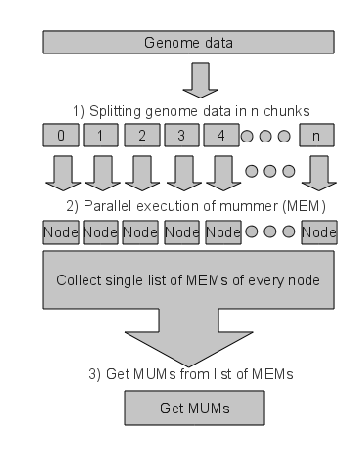
\epsfig{file=algorithm.eps,width=4.5cm,height=4cm} 
\end{center} 
\caption{Data-level parallelism technique for whole genome alignment.} 
\label{algorithm} 
\end{figure} 
The division of genome data was used using the paradigm of data-level parallelism which consists of a generation of chunks of a sequence with a fixed size and a fixed overlap. One issue arises when a genome is splitted because of the heuristic used in the algorithm is affected. So that, a longer sequence is more likely to have a better finding of MUMs while a smaller one can produce MUMs which are not effective MUMS.\\
Another consideration was the genome structure, because a genome is build from a finite alphabet $\Sigma=\{a,g,c,t,n\}$ but according to the MUMmer's algorithm each alignment is made using only the nucleotide base pairs, this means that letter "n" in a biological way can mean anything: (a,g,c,t). A complex structure of a genome can have a huge impact of our data level parallelism.\\
%The main idea in MUMmer is its heuristic, Maximal Unique Match (MUM), based on this concept it is possible to cover a huge region of a genome when reference and query genomes are very closely related. However 
To get a MUM, it requires an important feature its uniqueness. 
%We had to face with concept while we evaluated different ways to implement the data-level parallelism. 
Uniqueness can only be found when a whole genome is checked.
%if some part of it is only evaluated we could miss the rest of the genome. 
In other words, after finding MUMs within a chunk it is not possible to determine if the MUM found is or not a "unique" MUM, globally in the genome,  because these MUMs are unique only in the chunk that has been read, the rest of the genome it is not known.\\
One solution to solve this problem is to drop the MUMmer's heuristic in order to be able to find the correct MUMs when we apply our data-level parallelism. The new approach is to find a Maximal Exact Match (MEM), a MEM allows to drop the uniqueness of a match but with a high computational cost: a brute-force approach.\\
%A MEM as shown in Figure \ref{mem} has the advantage of getting the true MUMs regardless a division of genome data. In Figure \ref{mem} R stands for reference genome and Q stands for query genome, this example shows that blue and red matches have exact matches but turn out not to be unique, then not a valid MUM; a true MUM is the green match.\\
Nevertheless, the major problem with the use of MEM is that the number of occurrences increases exponentially when \emph{shorter MEM} are used. Moreover, the high ratio of MEMs requires to save them in some place, memory or disk, that means a heavy use of resources in both CPU and Memory. This drawback is the main disadvantage because the hits of MEMs are increasing with the size of the genome. A new phase has to be designed to reduce the use of resources when a short MEM is searched.
%\begin{figure}[htb] 
%\begin{center} 
%  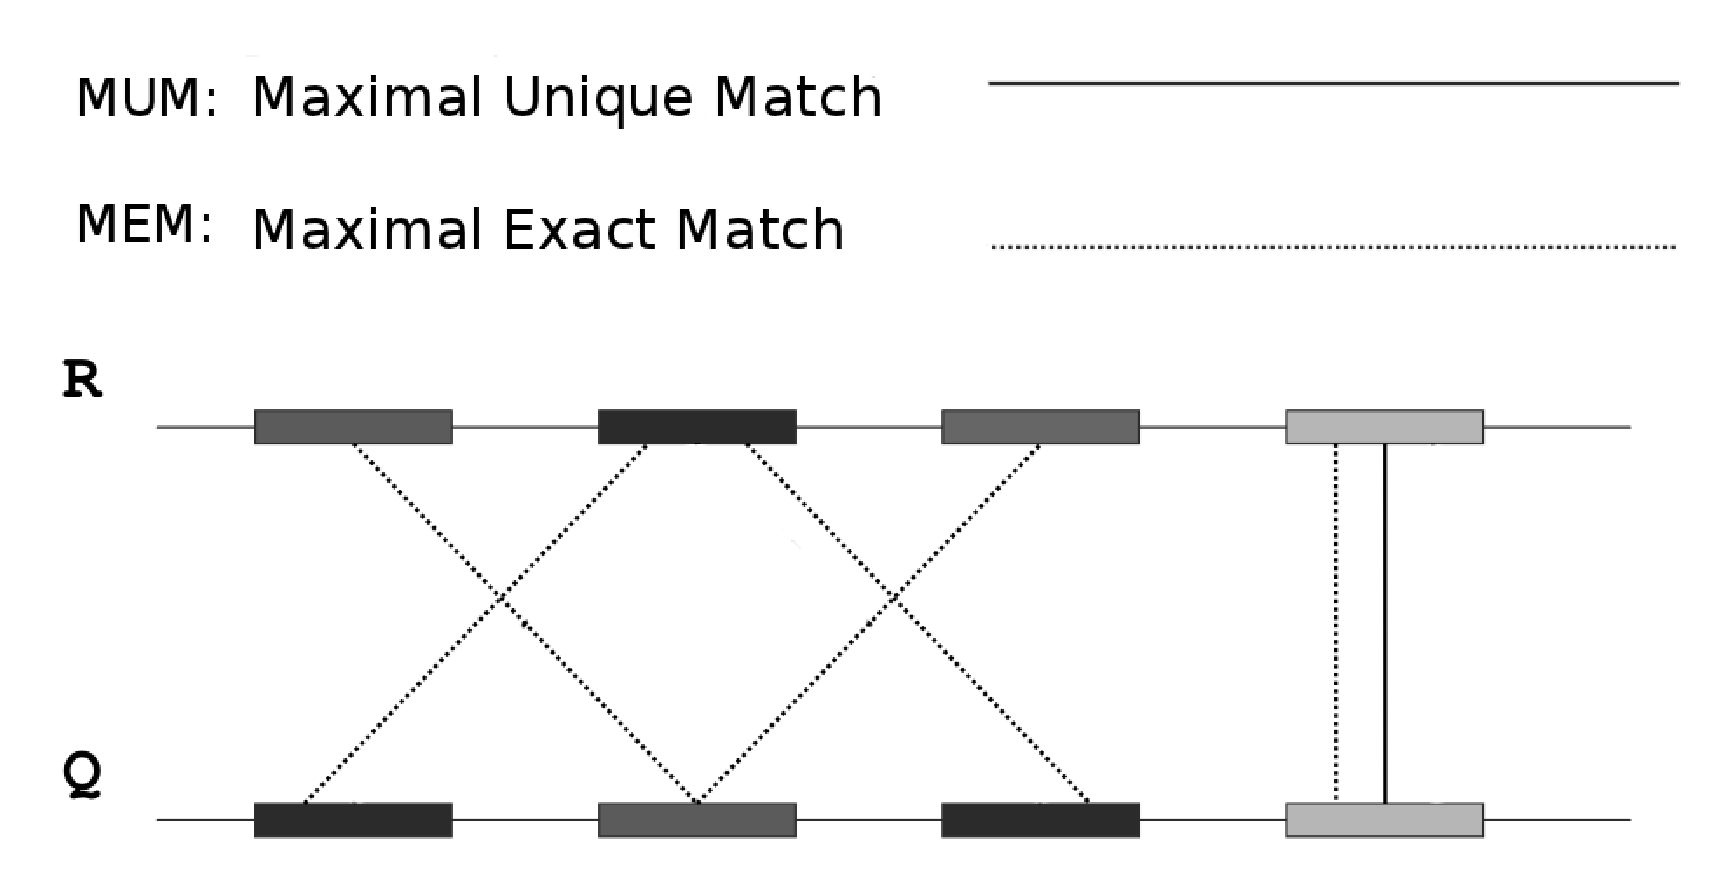
\epsfig{file=mem.eps,width=6cm, height=3cm} 
%\end{center} 
%\caption{Types of matches}
%\label{mem} 
%\end{figure} 
\section{Implementation} 
\label{implementation}
%When there is only one query sequence, one can try to split the query sequence and assign each part to a processor. This part covers in detail every aspect of Xipe Totec.
This section explains in detail how our proposal is implemented and the modifications in order to be executed in MUMmer. The following diagram, see Figure \ref{xipe-totec}, shows the add-ons of our approach, one is executed before MUMmer and the another after MUMmer.
\begin{figure}[htb]  
 \begin{center} 
    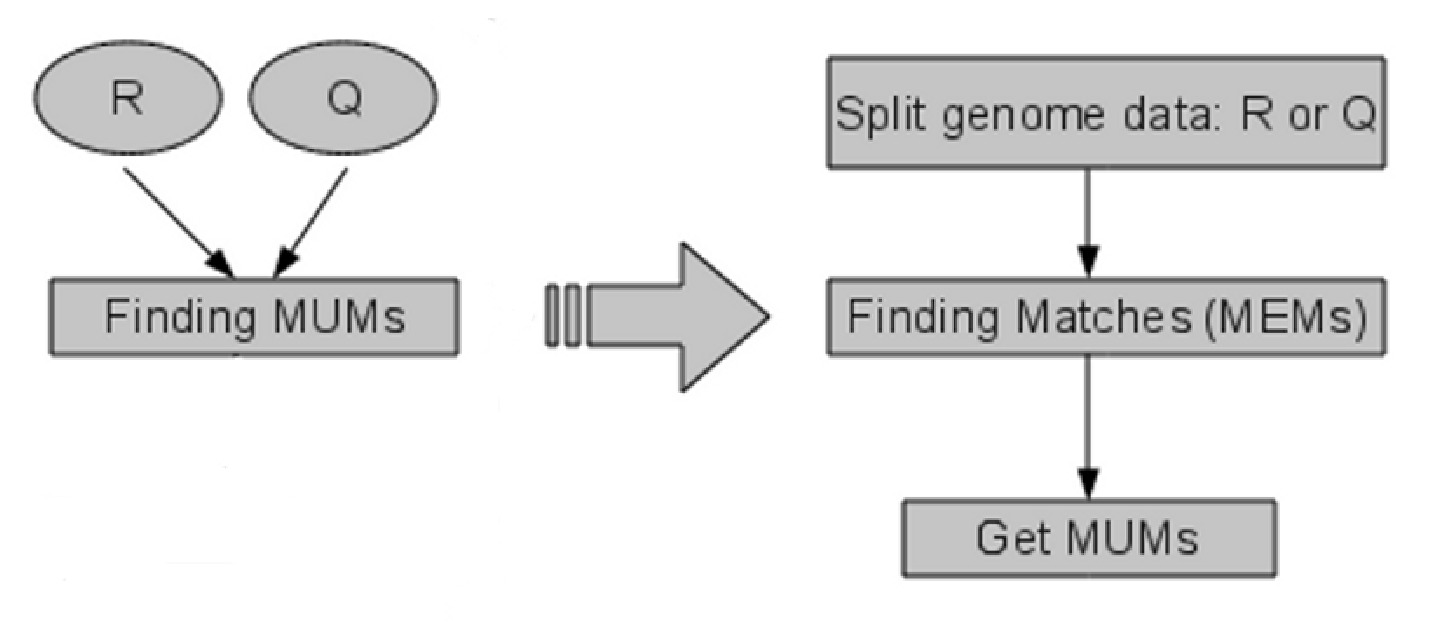
\epsfig{file=xipe-totec1.eps,width=7.5cm} 
 \end{center}
 \caption{Xipe Totec: proposal for parallelization of whole genome alignment} 
 \label{xipe-totec} 
\end{figure}
The following sections explain how the split of genome data, search of MEMs and get MUMs are carried out in our proposal.
\subsection{Split genome data} 
As it was previously explained, the approach is to use a fixed size division of genome data in as many chunks as  many available cores. Xipe Totec needs to know how many cores will be used in order to divide the genome data.\\
One key aspect of Xipe Totec is the way to split a genome. To align a genome requires a reference genome so that, there are two ways of using Xipe Totec:
\begin{itemize}
\item Splitting reference genome.
\item Splitting query genome.
\end{itemize}
Both of them can reduce the computation time or memory usage.\\
To split genome data a perl script was coded to do this task, the script requires the following arguments:
\begin{itemize}
\item Genome data to be splitted.
\item Number of chunks.
\item Overlap size.
\item Location to save the genome data.
\end{itemize}
\subsection{Finding MEMs}
This phase requires the mummer program, one of the several small programs in the MUMmer suite. mummer has several options.
In order to get a correct alignment, our proposal requires to compute MEMs instead of MUMs, so that mummer is executed with:
\begin{itemize}
  \item -n: to match only nucleotides.
  \item -maxmatch: option to get MEMs.
  \item -l \emph{length}: to find MEMs of a some minimum length.
\end{itemize}
List of MEMs is saved to a file which has the following format:
\begin{verbatim}
>Information about the sequence
Position_in_R Position_in_Q Length_of_MEM
\end{verbatim}
This list has to be joined with the output of every chunk computed and then the whole list is  manipulated in the following phase, \ref{getting}.
\subsection{Getting MUMs}
\label{getting}
This is the most important phase in our approach because it outputs the final list of MUMs those that are the same to the serial execution of mummer.\\
This phase needs the list of MEMs to process them and find those matches that are unique. The following diagram shows the basic idea behind this phase, see Figure \ref{xt}.
\begin{figure}[htb]  
 \begin{center} 
   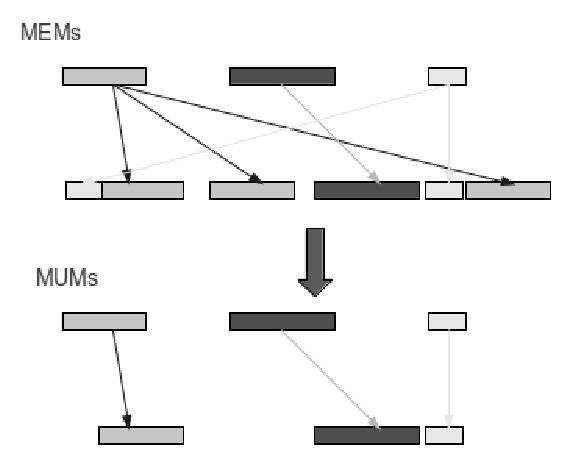
\epsfig{file=xt.eps,width=5cm, height=2cm} 
 \end{center} 
 \caption{Xipe Totec: Finding the real MUMs} 
   \label{xt} 
\end{figure}
To get the MUMs we filter those MEMs that are unique in the list and order them using a modified version of LIS\footnote{Longest Increasing Subsequence} algorithm.
The algorithm is shown below:
\begin{algorithmic}
\STATE{Input: List of MEMs: Position in R, position in Q, length of MEM}
\STATE{Sort MEMs by increasing position and decreasing length in R}
\FOR{$i:=0$ to $n$ in Total\_MEMs}
\IF{MEM[$i$] is not unique}
\STATE{Sort this subset by increasing position in Q and pick up the first MEM and drop the rest}
\ELSE {}
\STATE{MEM[$i$] is a MUM}
\ENDIF
\ENDFOR
\STATE{Sort MEMs by increasing position and decreasing length in Q}
\FOR{$i:=0$ to $n$ in Total\_MEMs}
\IF{MEM[$i$] is not unique}
\STATE{Sort this subset by increasing position in R and pick up the first MEM and drop the rest}
\ELSE {}
\STATE{MEM[$i$] is a MUM}
\ENDIF
\ENDFOR
\end{algorithmic}
The output of this algorithm gives the MUMs.
\section{Experiments and results}
To verify that our approach, Xipe Totec, can align a whole genome a set of tests were analyzed. These tests were carried out in a cluster with the following features:
\begin{itemize}
\item Hardware: 
\begin{itemize}
\item Processor Dual-Core Intel(R) Xeon(R) CPU 5160 @ 3.00GHz 4MB L2 (2x2)
\item Number of processors: 2
\item RAM: 12 GB Fully Buffered DIMM 667 MHz
\end{itemize}
\item  Software:
\begin{itemize}
\item Linux Kernel 2.6.16.46-0.12-smp x86\_64 GNU/Linux
\item gcc 4.3.2
\item MUMmer 3.22
\item Perl 5.8.8
\end{itemize}
\end{itemize}
Previously it was described two ways of parallelization. So that each genome alignment was executed following these phases:
\begin{itemize}
\item Split genome data:
\begin{itemize}
\item Genome size: 115,86 Mbp\footnote{Two nitrogenous bases paired together in double-stranded DNA by weak bonds; specific pairing of these bases (adenine with thymine and guanine with cytosine) facilitates accurate DNA replication; when quantified (e.g., 8 bp), refers to the physical length of a sequence of nucleotides \cite{ncbi}}.
\item Division of genome in 2, 4, 8, 16 chunks.
\item An overlapping size of 5000bp.
%  \begin{enumerate}
%    \item 100 Kbp
%    \item 250 Kbp
%    \item 500 Kbp
%    \item 2500 Kbp
%    \item 5000 Kbp
%  \end{enumerate}
\end{itemize}
\item Test for several size of MEMs:
  \begin{enumerate}
    \item 20 bp
    \item 50 bp
    \item 100 bp
    \item 500 bp
    \item 1000 bp
  \end{enumerate} 
\end{itemize}
Then each way of parallelization is executed:
\begin{itemize}
\item Align the query genome by splitting it against a global whole reference genome, see Figure \ref{splitqry}.
\begin{figure}[htb] 
  \begin{center}
    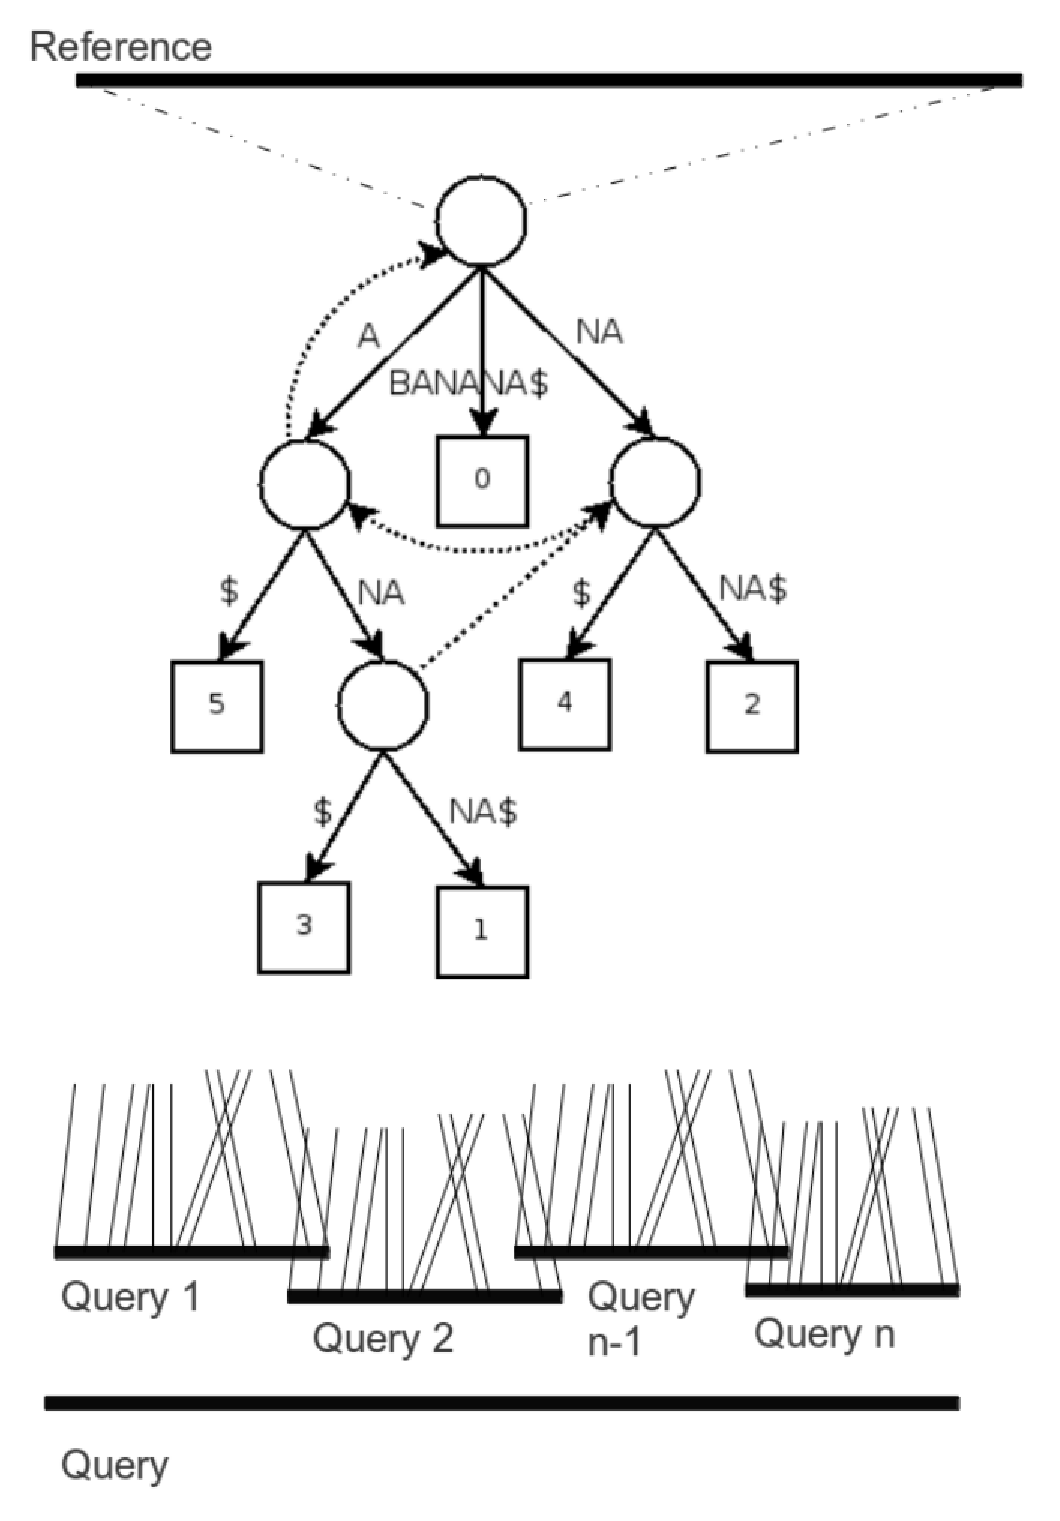
\epsfig{file=split_qry.eps,width=5cm,height=4cm}
  \end{center}
 \caption{Split query genome.}
 \label{splitqry}
\end{figure}
\item Align the whole query genome against every chunk of reference genome, see Figure \ref{splitref}.
\begin{figure}[htb]
  \begin{center}
    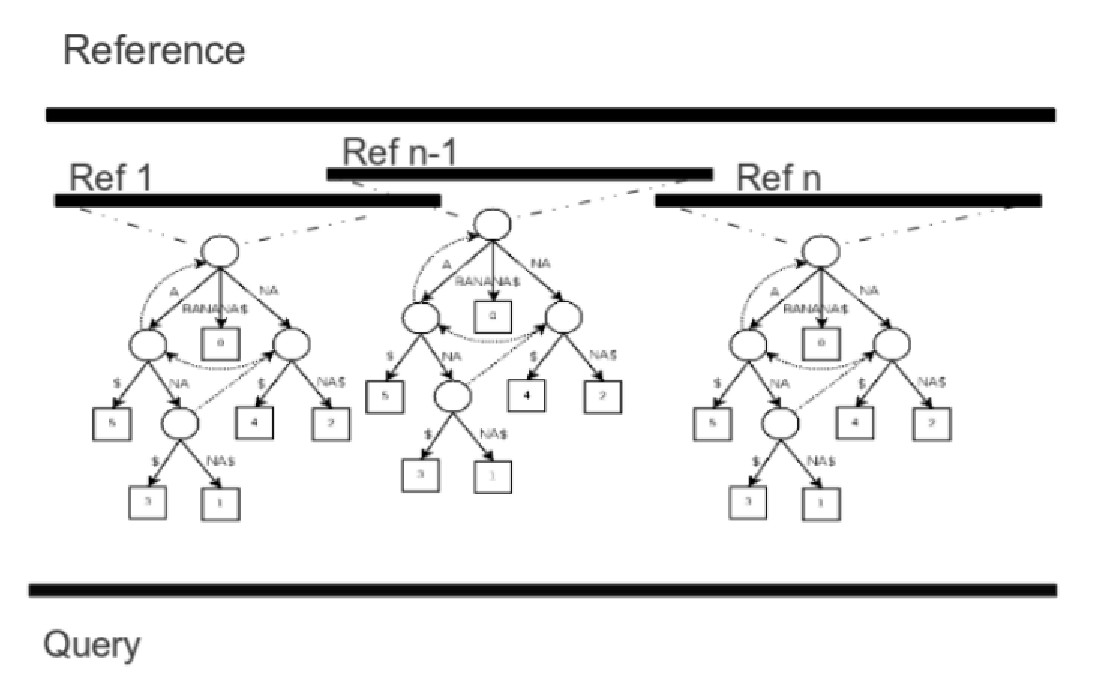
\epsfig{file=split_ref.eps,width=7.5cm}
  \end{center}
 \caption{Split reference genome.}
 \label{splitref}
\end{figure}
\end{itemize}
Our was with the human chromosome 13 as reference genome and the chimpanzee chromosome 13 as query genome. The correct size of each genome is:
\begin{itemize}
  \item Human chromosome 13: 95.78 Mbp
  \item Chimpanzee chromosome 13: 115,86 Mbp
\end{itemize}
The first parameter to measure was the construction of suffix tree. In Figure \ref{hspan_st_r} is shown how, a division of reference genome improves the building time of suffix tree, up to 27 times when the reference is divided in 16 chunks. Though a quick build of suffix tree is achieved when the reference is split the but this improvement is not possible when the query genome is split, in Figure \ref{hspan_st_q} is shown the building time for suffix tree which remains constant.
\begin{figure}[htb] 
\centering
\subfloat[][Construction of ST split Human Chr13 reference.]
{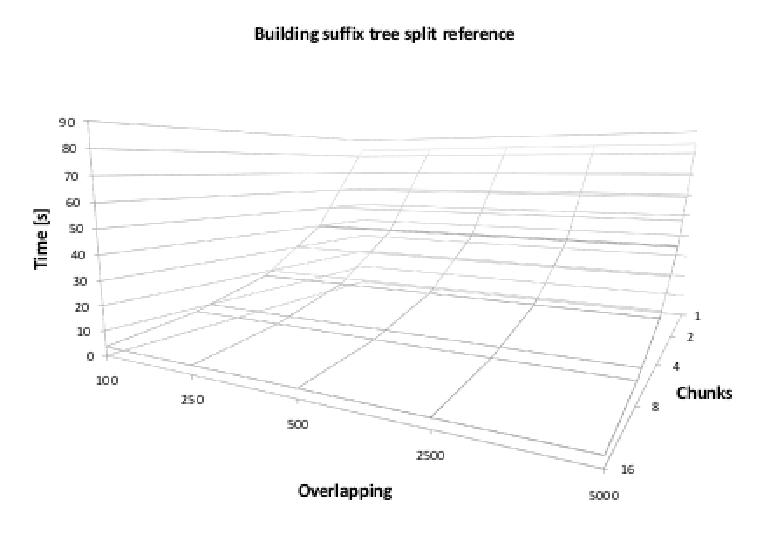
\epsfig{file=hspan_st_r.eps,width=3.4cm} \label{hspan_st_r}}
\hspace{0.1cm}
\subfloat[][Construction of ST split Chimpanzee Chr13 query.]
{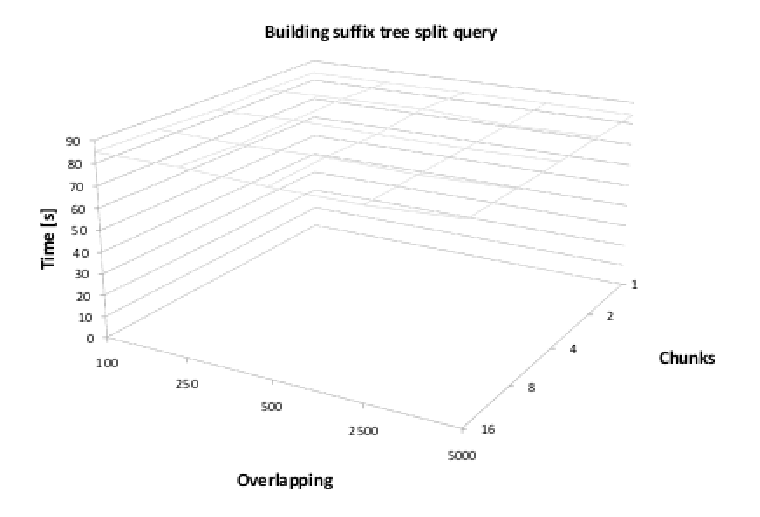
\epsfig{file=hspan_st_q.eps,width=3.4cm} \label{hspan_st_q}}
\end{figure}
The second parameter to test was the computation time to find the MEMs. As it was explained in the previous chapter we follow a brute-force approach to get the same list of MUMs when our technique is used. In other words, it might be possible that for some genome sizes our approach can be worse than the sequential version.\\
In the Figure \ref{hspan_find_r_5000} is shown the several configurations tested when the reference genome is split. \\
It is important to point out that this test shows that for some configurations our approach does not work at all: when the Match length is very short, like 20 bp. The answer to this problem is that when a small match is searched in a big genome the number of matches can become exponentially. This undesirable feature can be seen in Figure \ref{hspan_drop} and Figure \ref{hspan_mums} which shows the high number of hits when a short match is searched.\\
\begin{figure}[htb] 
\centering
\subfloat[][Finding MEMs split Human Chr13, Overlap=5000bp.]
{\epsfig{file=hspan_find_r_5000.eps,width=3.2cm} \label{hspan_find_r_5000}}
\hspace{0.1cm}
\subfloat[][Finding MEMs split Chimpanzee Chr13, Overlap=5000bp.]
{\epsfig{file=hspan_find_q_5000.eps,width=3.2cm} \label{hspan_find_q_5000}}
\end{figure}
On the other hand when the query genome is split the reduction of time to find MEMs is only of the magnitude of 20\%.\\
Memory usage is a big issue when a genome goes from a few Mbp to hundreds of Mbp, our reference genome is almost 100Mbp and the requirement for memory can be seen in Figure \ref{hspan_ram}. For a genome of 95Mbp, the algorithm requires more than 1.6GB, from our experiments we can show that if we divide genome reference in 16 chunks, memory requirement reduces to only 12.5\% of the sequential version use of memory.\\
\begin{figure}[htb] 
\begin{center}
      \epsfig{file=hspan_ram.eps,width=7.5cm}
    \caption{Use of memory when aligning Human Chr13 vs. Chimpanzee Chr13.}
    \label{hspan_ram}
  \end{center}
\end{figure}
The most important step in our test was to verify that our parallelization can get the same alignment (same list of MUMs from the sequential version), in Figures \ref{hspan_mums}, \ref{hspan_mums_20}, \ref{hspan_mums_50}, \ref{hspan_mums_100}, \ref{hspan_mums_500} and \ref{hspan_mums_1000} reader can watch the list of MUMs which should be the same when we apply our parallelization technique. In order to know if our approach does the job we filter those matches which are MUMs. To understand this point, the Figure \ref{hspan_drop} shows the number of matches discarded.
\begin{figure}[htb] 
\centering
\subfloat[][List of MUMS for several sizes of MUM when aligning Human Chr13 vs. Chimpanzee Chr13.]
{\epsfig{file=hspan_mums.eps,width=3.2cm} \label{hspan_mums}}
\hspace{0.1cm}
\subfloat[][Percentage of dropped MEMs in order to get the same list of MUMs for the sequential version of MUMmer, when aligning Human Chr13 vs. Chimpanzee Chr13.]
{\epsfig{file=hspan_drop.eps,width=3.2cm} \label{hspan_drop}}
\end{figure}
\begin{figure}[htb] 
\centering
\subfloat[][Frequency of MUMs, length of 20bp, found when aligning Human Chr13 vs. Chimpanzee Chr13.]
{\epsfig{file=hspan_mums_20.eps,width=3.2cm} \label{hspan_mums_20}}
\hspace{0.1cm}
\subfloat[][Frequency of MUMs, length of 50bp, found when aligning Human Chr13 vs. Chimpanzee Chr13.]
{\epsfig{file=hspan_mums_50.eps,width=3.2cm} \label{hspan_mums_50}}
\end{figure}
\begin{figure}[htb] 
\centering
\subfloat[][Frequency of MUMs, length of 100bp, found when aligning Human Chr13 vs. Chimpanzee Chr13.]
{\epsfig{file=hspan_mums_100.eps,width=3.2cm} \label{hspan_mums_100}}
\hspace{0.1cm}
\centering
\subfloat[][Frequency of MUMs, length of 500bp, found when aligning Human Chr13 vs. Chimpanzee Chr13.]
{\epsfig{file=hspan_mums_500.eps,width=3.2cm} \label{hspan_mums_500}}
\end{figure}
\begin{figure}[htb] 
\centering
\subfloat[][Frequency of MUMs, length of 1000bp, found when aligning Human Chr13 vs. Chimpanzee Chr13.]
{\epsfig{file=hspan_mums_1000.eps,width=3.2cm} \label{hspan_mums_1000}}
\end{figure}
\section{Conclusions}
We have set in place a parallelization of whole genome alignment, Xipet Totec, and used MUMmer to evaluate the alignment of two genomes. We have found that a data level parallelism allows an approximation of a correct alignment.\\
We view this work as a starting point toward the goal of completely automating alignment parallelization. In addition to split data genome, we will also need to automatically choose seeding strategies and thresholds. \\
This work has made some progress, especially in improved pairwise alignment with a heuristic basis, which has shown the efficiency to handle memory management and the parallel distribution of genome data in order to get a quicker whole genome alignment. Additionally, a better heuristic should be used to allow the full use of clusters and multicore architectures. This new heuristic may improve the finding of matches so that every process can handle its chunk and it could notice if a match is unique or not by checking the other chunks. In this way a new concept of distributed MUM is defined:
\begin{center}
\begin{mydef}
Distributed Maximal Unique Match(DMUM) substring is a common substring of the two genomes that is longer than a specific minimum length d such that it is maximal, that is, it cannot be extended on either end without incurring a mismatch and it is unique in any of the chunks of the genome.
\end{mydef}
\end{center}
DMUM works by checking first if it is a MUM locally and then asking to the other chunks if this MUM is a real MUM in the whole genome. The DMUM has the advantage of having less intermediate data (MEMs) but with an overhead of communications between each chunk and the computation time to check if the match is unique or not.\\
Our technique is a startup to explore the multiple faces of bioinformatics to do a better use of the available computer resources. This work shows that a novel parallelization and the knowledge of genome data can improve the run time and memory.\\
Several configurations were tested and some drawbacks were found. The main restriction to implement this technique  is the  limited memory resource in our environment test.
\subsection{Drawbacks}
Our novel approach has some limitations which are listed below:
\begin{itemize}
  \item It can work well with genome data of size less than 100Mbp.
  \item The use of a short match length can heavily impact in performance of our approach.
  \item This technique does not provide any feature of checkpoint.
  \item Our approach does not take advantage of any parallel programming language (OpenMP, OpenMPI, etc.).
\end{itemize}
These drawbacks are some opportunities to work with in the near future.\\
In addition, there are more issues related to computational tasks like a fair usage of available resources to do whole genome alignment. Among the desirable attributes any whole genome alignment algorithm should have are:
\begin{itemize}
\item Time: in order to be able to process whole genomes.
\item Space: a clever use of data structures to not run out of memory. 
\end{itemize}
Both of these attributes were enhanced in MUMmer to provide a first approach to whole genome alignment in HPC clusters.
\section*{Acknowledgements}
This work was supported by grant from Ejecuci\'on eficiente de aplicaciones multidisciplinares: nuevos desaf\'ios en la 
era multi/many core, with reference TIN2011-28689-C02-01.
 
\nocite{*}
\bibliographystyle{Jornadas}
\begin{thebibliography}{1}
\bibitem{Mummer1}
   Arthur L Delcher and Simon Kasif and Robert D. Fleischmann and Jeremy
    Peterson and Owen white and Steven L. Salzberg,
   \newblock{\em Alignment of whole genomes},
   \newblock Nucleic Acids Research, 1999
\bibitem{mummer2}
   Arthur L. Delcher and Adam Phillippy and Jane Carlton and Steven
    L. Salzberg,
   \newblock{\em Fast algorithms for large-scale genome alignment and comparison},
   \newblock Nucleic Acids Research, 2002
\bibitem{Mummer3}
   Stefan Kurtz and Adam Phillippy and Arthur L Delcher and Michael
    Smoot and Martin Shumway and Corina Antonescu and Steven L. Salzberg,
   \newblock{\em Versatile and open software for comparing large genomes},
   \newblock Genome Biology, 2004
\bibitem{McCreight:1976:SST:321941.321946}
   McCreight, Edward M.,
   \newblock{\em A Space-Economical Suffix Tree Construction Algorithm},
   \newblock J. ACM, 1976.
\bibitem{Needleman1970General}
   Needleman, S. B. and Wunsch,
   \newblock{\em A general method applicable to the
search for similarities in the amino acid sequence of two proteins.},
   \newblock Journal of molecular biology, 1970.
\bibitem{Waterman}
   Smith, T. F. and Waterman, M. S.,
   \newblock{\em Identification of common molecular subsequences.},
   \newblock Journal of Molecular Biology, 1981.
\bibitem{ncbi}
   U.S. National Library of Medicine,
   \newblock Base pair
\bibitem{AVID}
   Bray, Nick Dubchak, Inna Pachter, Lior
   \newblock{\em AVID: A global alignment program.},
   \newblock Genome research, 2003
\bibitem{LAGAN}
   M. Brudno, C. Do, G. Cooper et al.
   \newblock{\em LAGAN and Multi-LAGAN : Efficient Tools for Large-Scale Multiple Alignment of Genomic DNA Outline of Algorithms},
   \newblock Genome research, 2003
\end{thebibliography}

\end{document}

